\xchapter{Use Example}{} %sem preambulo
\label{chap:useExample}

\acresetall 

\section{Scientific Method}\label{sec:method}

For this project development, the agile Scrum method has been used. In Scrum, projects are divided into cycles called sprints, with frequent meetings where the team can inform what is being done and think of ways to quickly improve the process. Scrum proposes constant project monitoring. Often the team will be meeting, exchanging experiences, evaluating what has been done and re-planning what will be done next.

During the requirements gathering, developers and other stakeholders sought to raise and prioritize the needs of future software users (referred as requirements). After the requirements gathering, in the requirements specification stage, developers made a detailed study of data collected in the previous activity, from where models were built to represent the software system being developed.

At the architectural design stage of the system two basic activities were performed: architectural design (or high level design), and detailed design (or low level design). Some aspects were considered at this stage of system design, such as: system architecture, platform used, Database Manager System (DBMS) used and graphical interface standard.

In the application development period, the backend and frontend components were created from the computational description of the design phase. Pre-existing software tools and class libraries were used to activity streamline. These tools and libraries were defined during the architectural design and were referenced in \cref{sec:WebAppFrondEnd,sec:WebAppBackEnd} .

For system validation, two main requirements were evaluated: the components and the behavior of who will use the application. For the first point, functional, integration and security tests will be performed. For the second, the \acf{TAM} method was used to evaluate user acceptance, utility and ease of use.

The appendix \ref{app:projectManagement} presents the activities for project management, the user stories and non-functional requirements. 


\section{Workflow}\label{sec:workflow}

The first step when creating a new Supply Chain  is to create and configure the asset. This action is made by the admin user. By going through the setup wizard, first the asset's info is requested:

\begin{figure}[H]
\begin{center}
  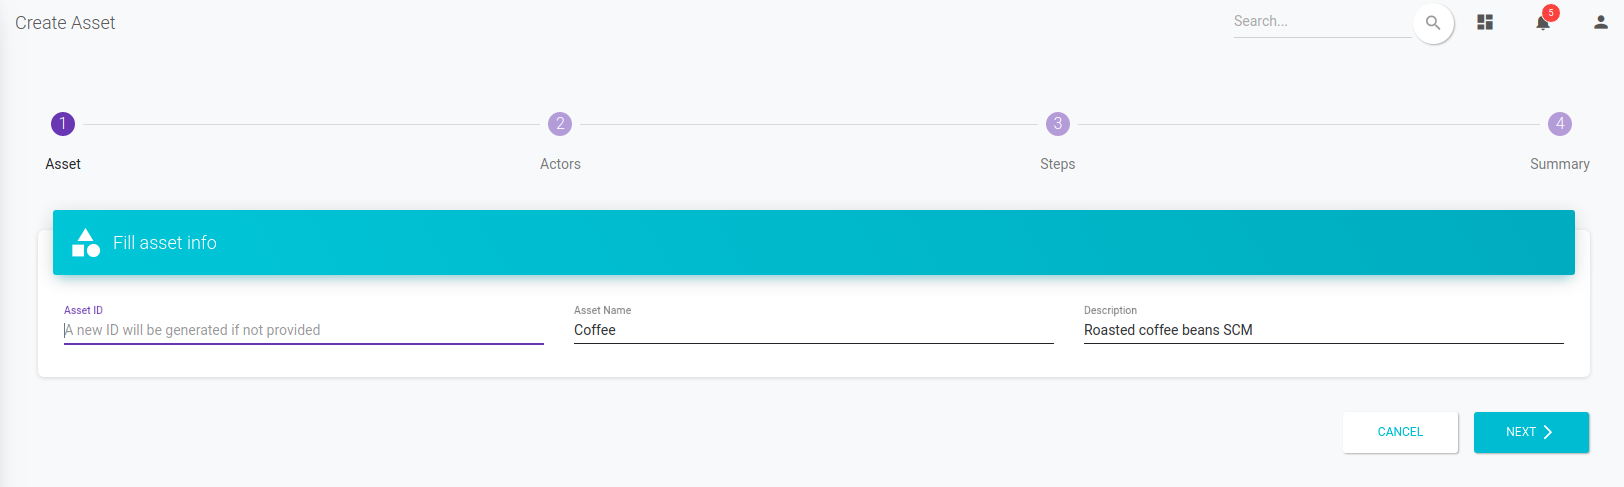
\includegraphics[scale=0.27]{images/use_example/01_create_asset_1.png}
\caption{Fill asset info.}
\label{fig:create_asset_1}
\end{center}
\end{figure}

Then the admin will add actors to the SCM informing its types:

\begin{figure}[H]
\begin{center}
  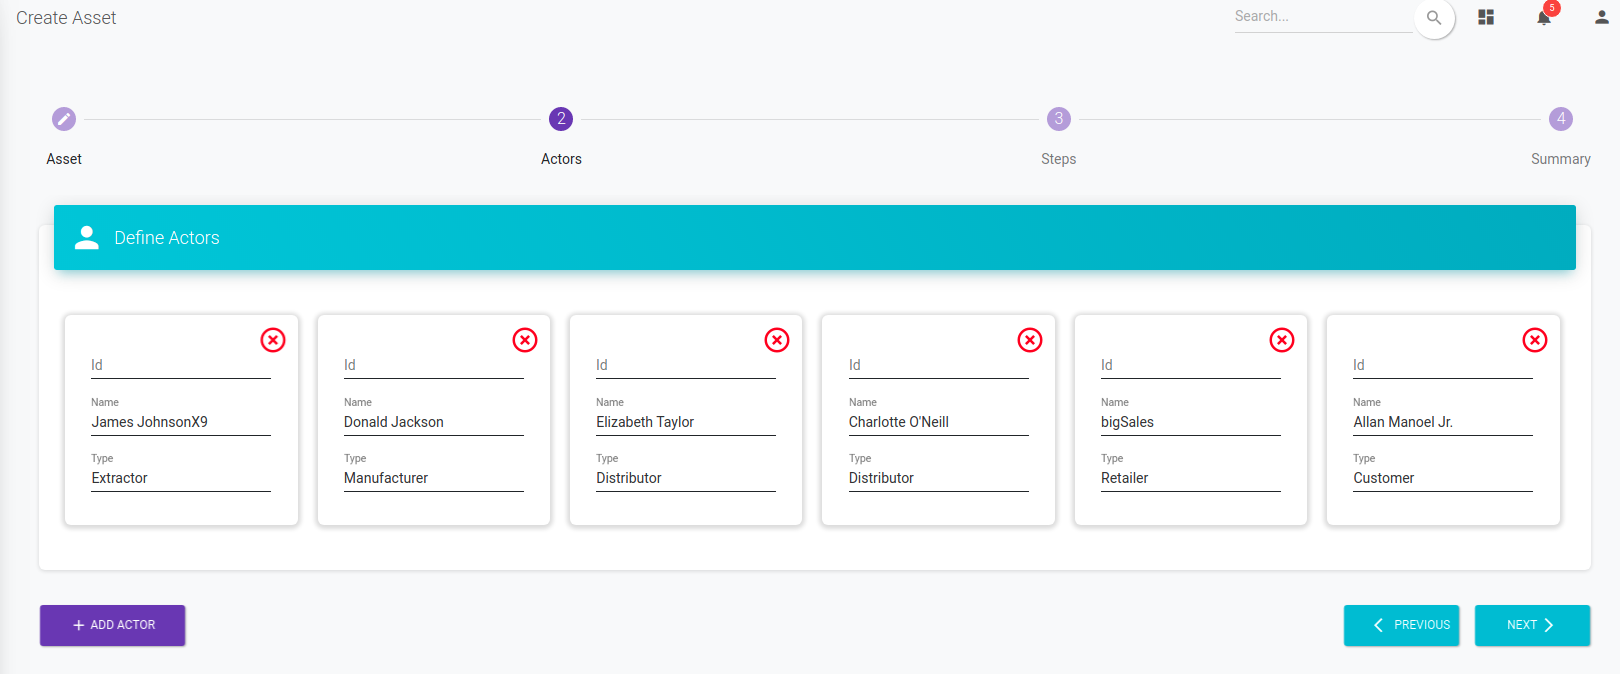
\includegraphics[scale=0.27]{images/use_example/02_create_asset_2.png}
\caption{Adding actors.}
\label{fig:create_asset_2}
\end{center}
\end{figure}


The next phase in the wizard is to define the Supply chain steps, specifying the order and binding it to the previous created actors' types:

\begin{figure}[H]
\begin{center}
  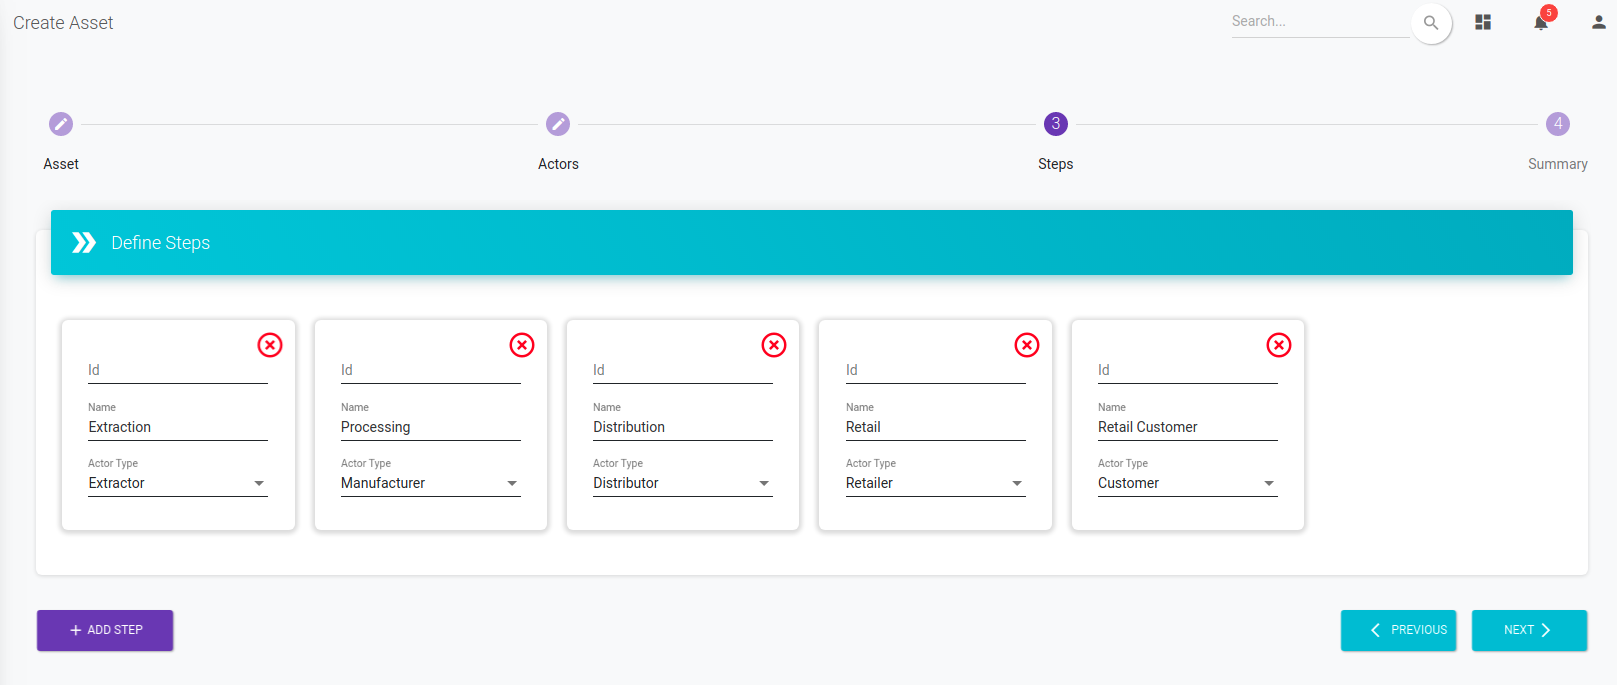
\includegraphics[scale=0.27]{images/use_example/03_create_asset_3.png}
\caption{Defining steps.}
\label{fig:create_asset_3}
\end{center}
\end{figure}

The final step, before submitting it, is to review all the information previously added in the review asset details page, under the wizard:
\begin{figure}[H]
\begin{center}
  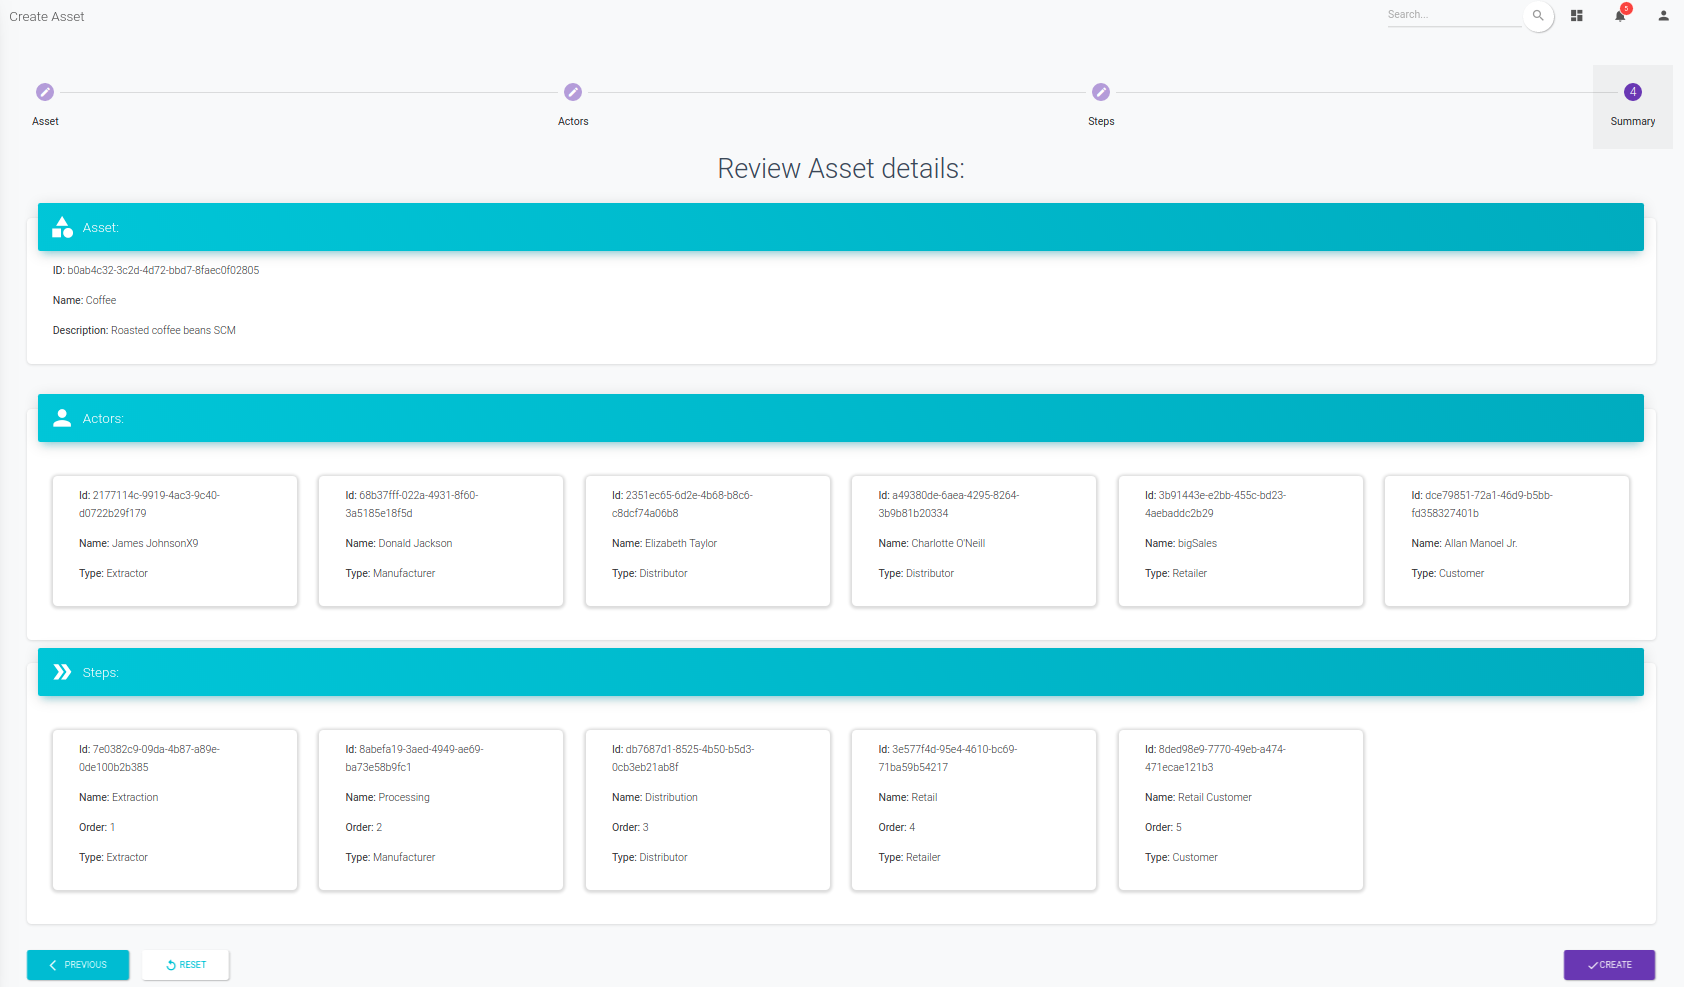
\includegraphics[scale=0.265]{images/use_example/04_create_asset_4.png}
\caption{Review asset details before submit.}
\label{fig:create_asset_4}
\end{center}
\end{figure}


Once created, the asset can be seen in the assets list, where the admin can perform crud operations by the actions items. When clicking in the asset details the current user is redirected to the asset details page where the main information about asset items, actors and steps can be seen. The card header contains a tab menu to provide navigation through these entities. 
% \begin{figure}[H]
% \begin{center}
%   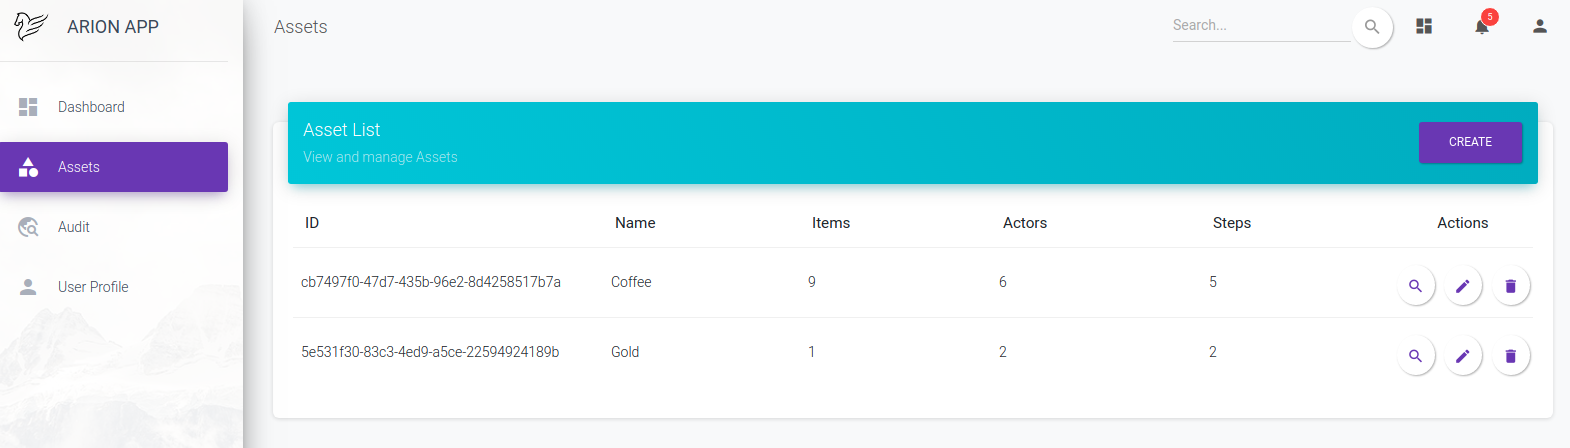
\includegraphics[scale=0.28]{images/use_example/05_asset_list.png}
% \caption{Asset list and action buttons.}
% \label{fig:asset_list}
% \end{center}
% \end{figure}



\begin{figure}[H]
\begin{center}
  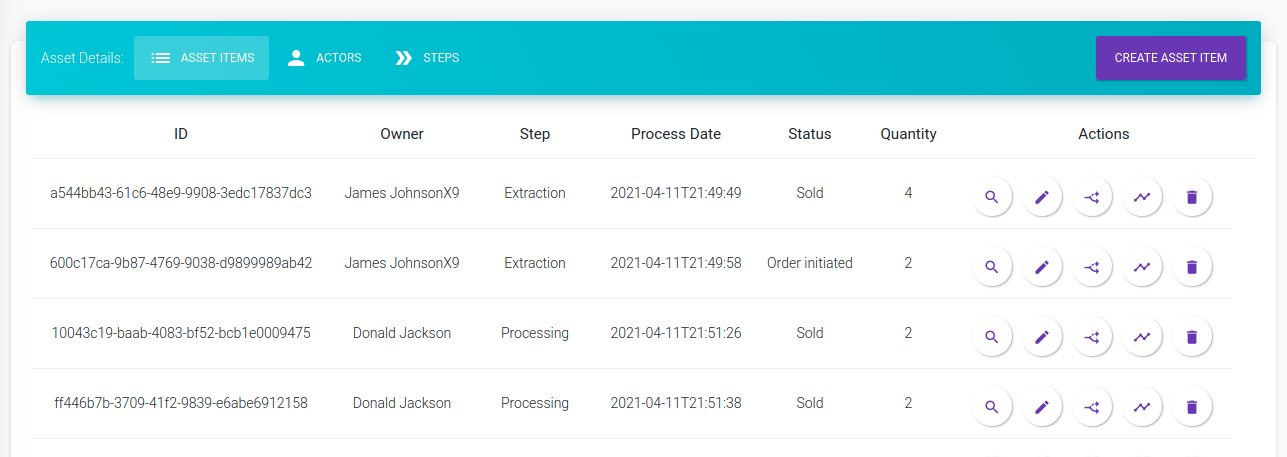
\includegraphics[scale=0.35]{images/use_example/06_asset_Item_list.png}
\caption{Asset Items list.}
\label{fig:asset_item_list}
\end{center}
\end{figure}

\begin{figure}[H]
\begin{center}
  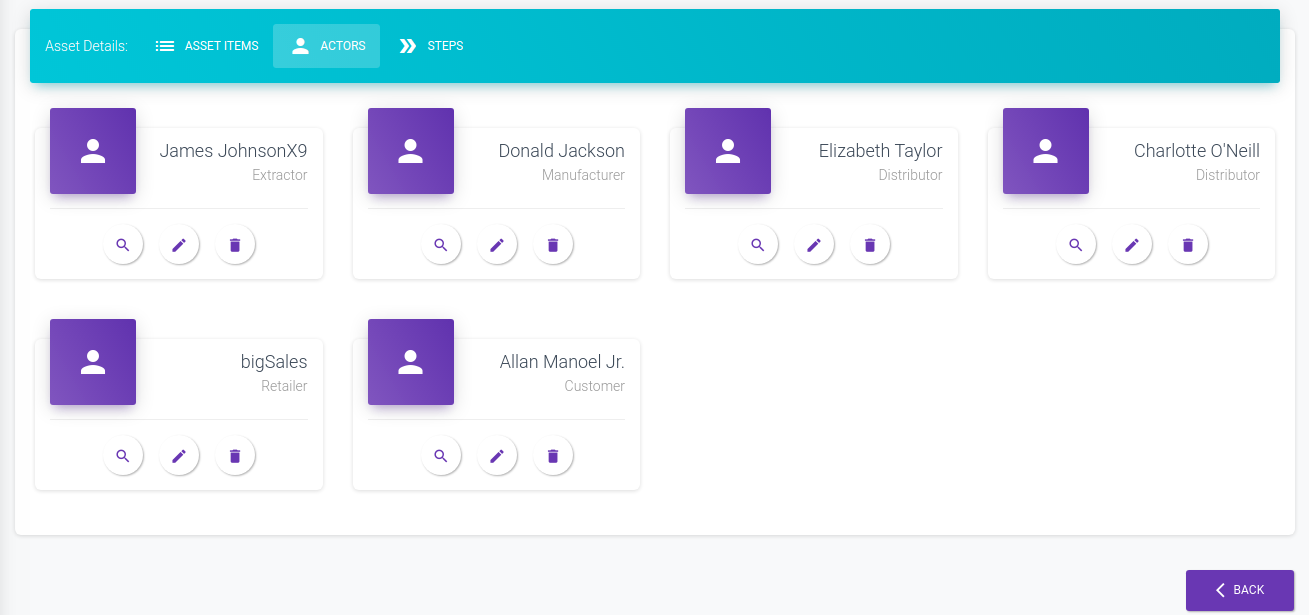
\includegraphics[scale=0.34]{images/use_example/07_actor_list.png}
\caption{Actors list.}
\label{fig:actor_list}
\end{center}
\end{figure}

\begin{figure}[H]
\begin{center}
  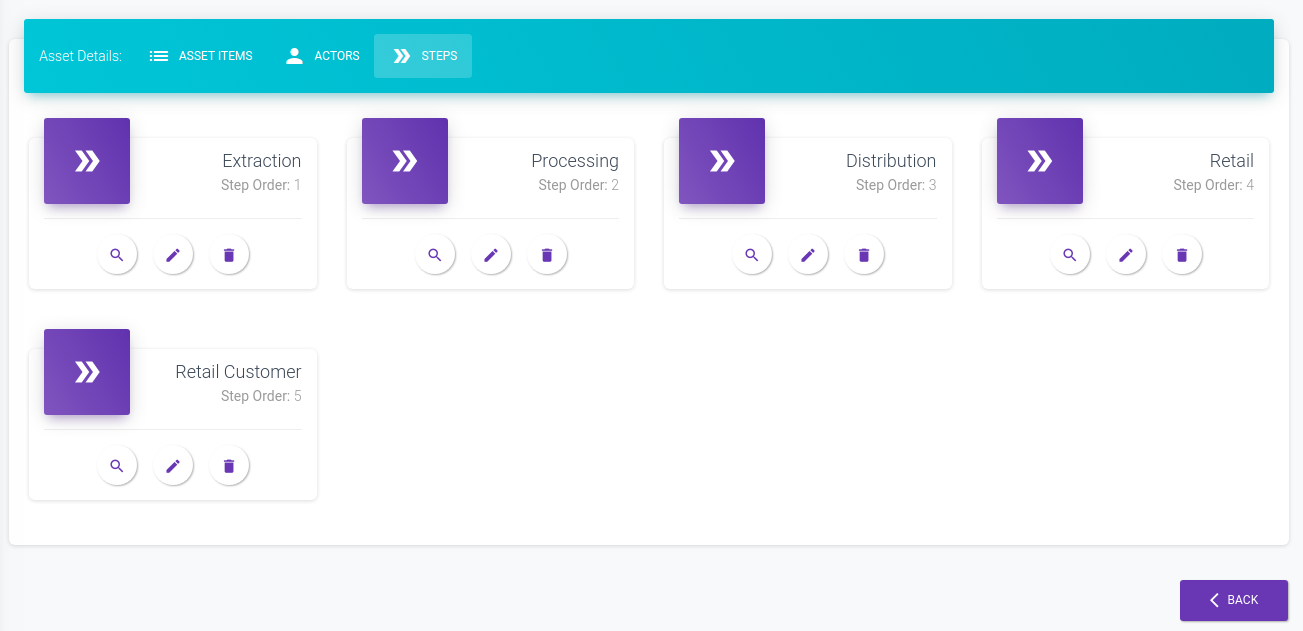
\includegraphics[scale=0.34]{images/use_example/08_steps_list.png}
\caption{Steps list.}
\label{fig:step_list}
\end{center}
\end{figure}

As admin there is also button actions to perform crud operations such as create an asset item which will redirect the user to the create asset item form: 

\begin{figure}[H]
\begin{center}
  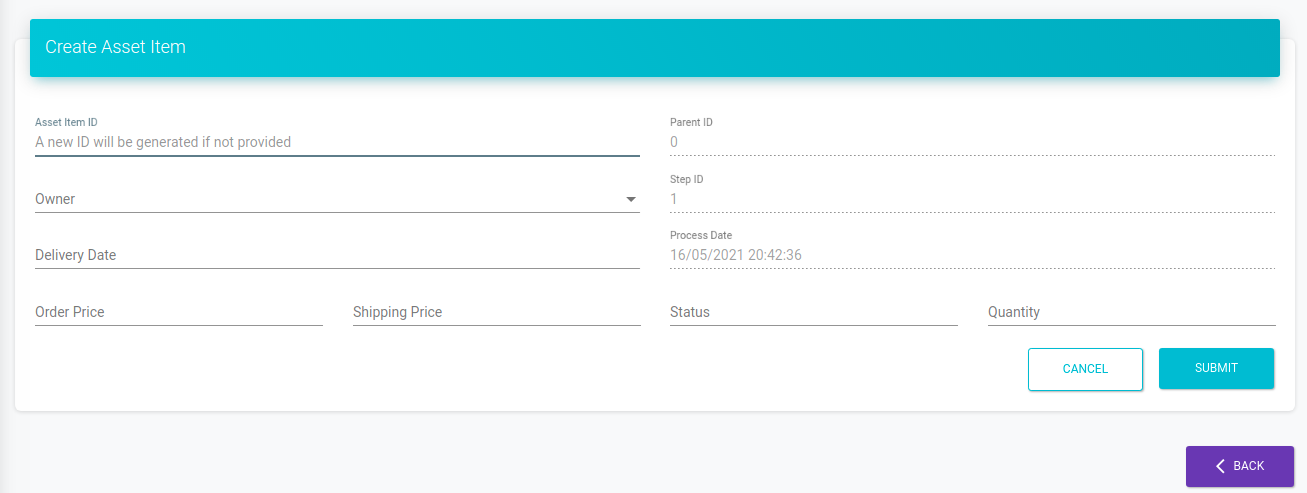
\includegraphics[scale=0.34]{images/use_example/09_create_asset_Item.png}
\caption{Create asset item form.}
\label{fig:create_asset_item}
\end{center}
\end{figure}


In the asset items list, beyond the crud actions there is also two new actions: move asset item and track asset item. The first one shows a form where the user can move an asset through the SCM steps. The user can only move this asset item to the next or the previous step in the supply chain. The second one displays the tracked info about the chosen asset item. It shows the children tree of the selected element and its ancestors.

\begin{figure}[H]
\begin{center}
  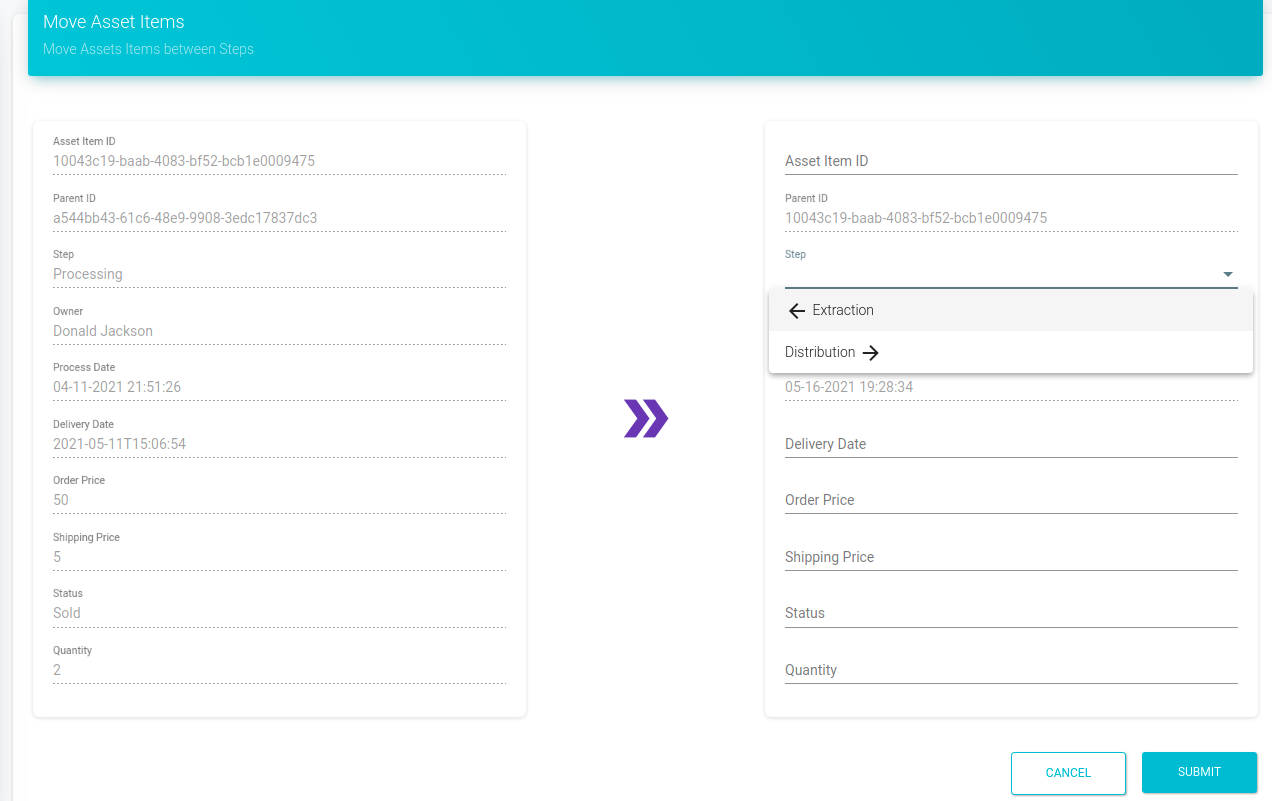
\includegraphics[scale=0.32]{images/use_example/091_move_asset_Item.png}
\caption{Move asset item form.}
\label{fig:move_asset_item}
\end{center}
\end{figure}

%

\begin{figure}[H]
\begin{center}
  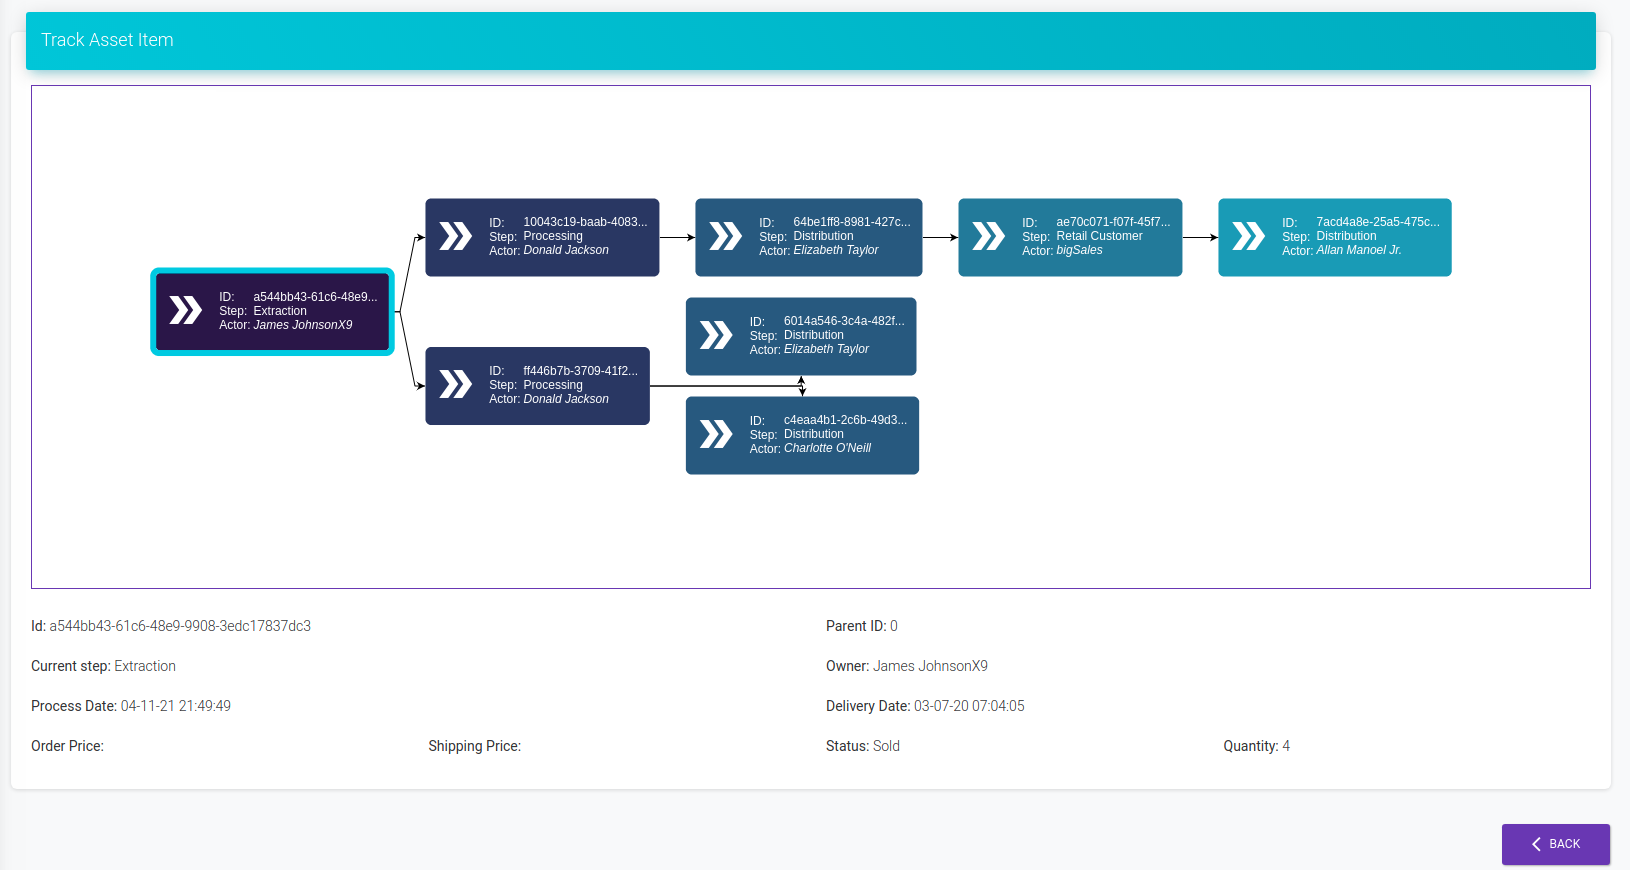
\includegraphics[scale=0.275]{images/use_example/092_track_asset_Item.png}
\caption{Track an asset item.}
\label{fig:track_asset_item}
\end{center}
\end{figure}

When clicking in a node in the chart, the information about the selected node is displayed under the diagram.